\section{Hardware}
\label{sec:hardware}

\subsection{Dron}
Para este desarrollo hemos elegido el dron 3DR Solo distribuido por la empresa norteamericana \url{https://3dr.com/}. Este dron se encuentra en una gama alta debido a sus capacidades \url{https://3dr.com/solo-drone/specs/}, tales como batería, distancia de comunicacion y potencia, cualidades que lo hacen un dron muy versatil. Durante el desarrollo se ha usado la versión oficial del software de 3DR 2.4.2. Se eligio esa debido a que era una versión estable y en versiones posteriores del software aun no se han corregido el principal fallo de conectividad debido a usar el mando como puerta de enlace.
A bordo de este dron se encuentra una placa Pixhawk 2, con la que nos debemos comunicar a traves del mando con el que se pilota el dron. Este inconveniente 3DR trata de solventarlo para evitar tener que usar el mando como enlace obligatorio. 

\begin{figure}[H]
  \centering
  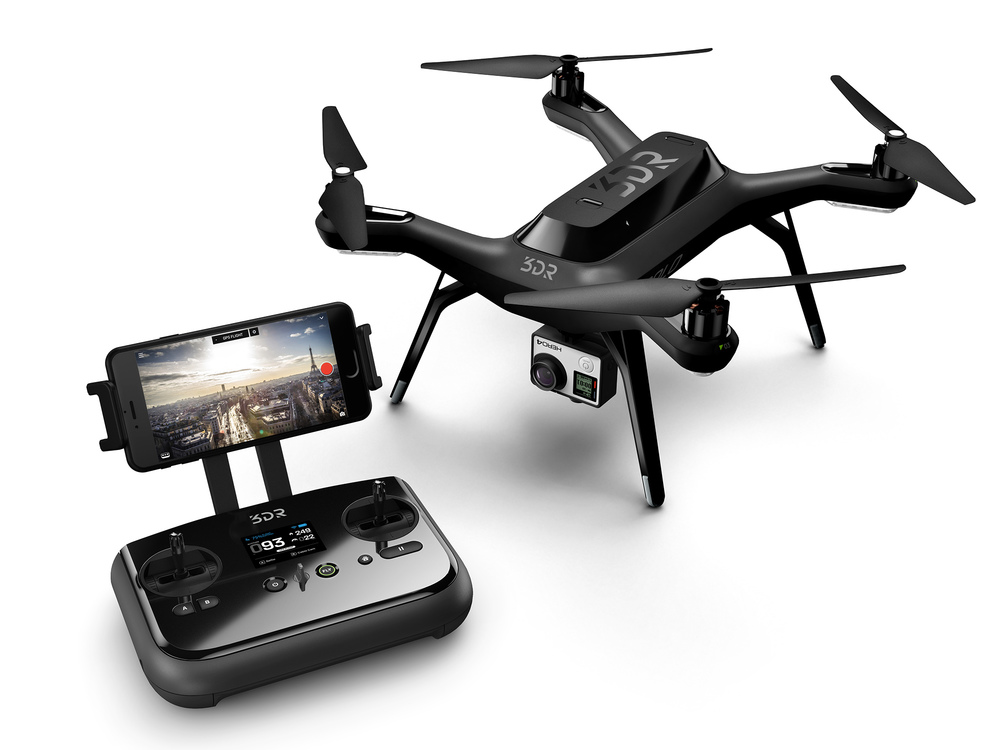
\includegraphics[scale=1]{imagenes/3drSoloDron.jpg}
  \caption{3DR Solo Drone}
  \label{fig:3drsolodrone}
\end{figure}


\cleardoublepage
\subsection{Pixhawk 2}

Esta placa se trata de un desarrollo especifico creado entre la "Pixhawk open hardware community" en colaboración con 3D Robotics y que vio como primer destinatario el 3DR Solo. Ofrece un interfaz que se apoya en comandos llamado MAVLink. A trav\'es de estos comandos se le puede tambi\'en enviar ordenes al piloto autom\'atico quien las ejecutar\'a más adelante trataremos el protocolo MAVLink en profundidad. El unico modo de conectarnos con el 3DR Solo sera a traves del mando, debido a que unicamente el mando es capaz de levantar la dirección IP a la que poder conectarnos. En posteriores evoluciones de la versión que controlan tanto el dron como el mando, desde los foros oficiales de 3DR, comentan que ya se aborda la solución de que sea el propio dron quien levante la dirección Ip a la cual poder conectarnos y no tener que depender del enlace del mando.

La comunicación entre el driver y el dron quedaría de la siguiente forma:

\begin{figure}[H]
  \centering
  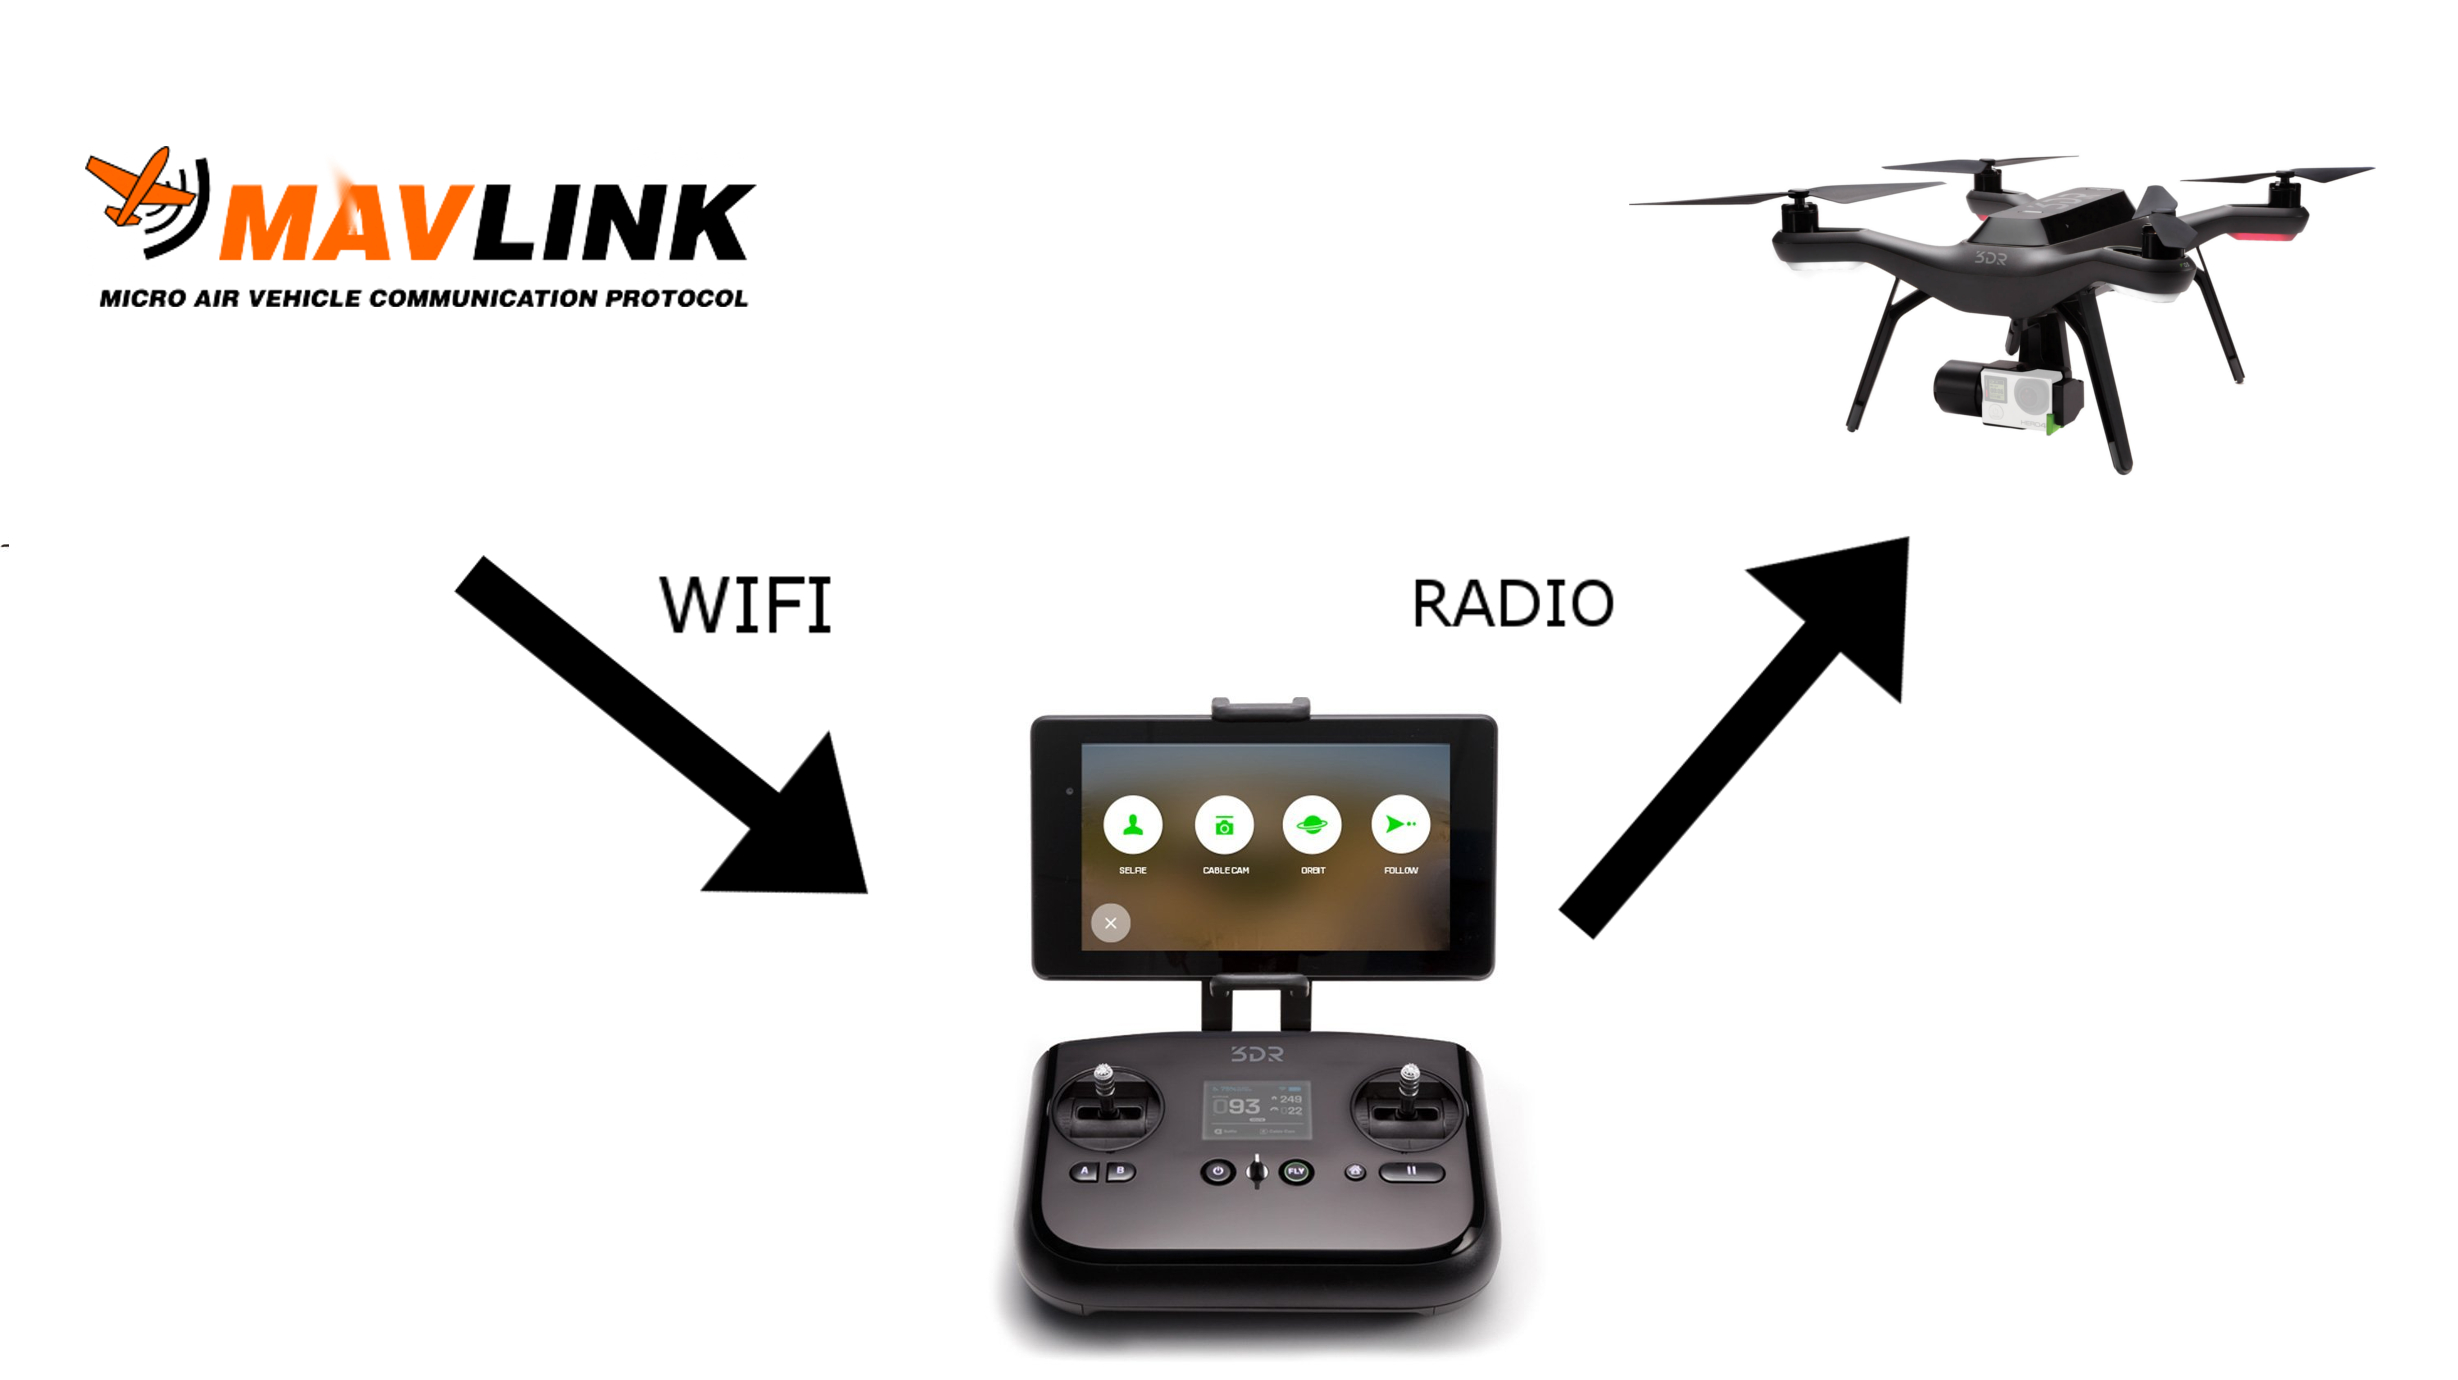
\includegraphics[scale=0.15]{imagenes/diagramaComunicacion.jpg}
  \caption{Diagrama comunicacion}
  \label{fig:diagrama}
\end{figure}

\section{Software}
\label{sec:software}

\subsection{JdeRobot}
\label{sec:jderobot}

JdeRobot es un framework desarrollado por el laboratorio de rob\'otica de la Universidad Rey Juan Carlos, para el desarrollo de aplicaciones de rob\'otica. Su última realease la 5.5 se liber\'o el 15 de Marzo de 2017 pudiendo ver los detalles de ésta en el github oficial\footnote{\url{https://github.com/JdeRobot/JdeRobot/wiki/JdeRobot-5.5.0}}.
JdeRobot se compone de interfaces, drivers, utilidades y aplicaciones para el desarrollo de cualquier proyecto de rob\'otica, se apoya en estos interfaces, algunos de ellos los veremos en profundidad a continuaci\'on, para interconectar entre sí todos los aplicativos del mismo y en Zeroc ICE para la comunicaci\'on entre ellos.
Algunos de los driver mas importantes que contiene serían:
\begin{enumerate}
\item MAVLinkServer. Desarrollado para intercomunicar JdeRobot con placas que utilicen el protocolo de comunicaci\'on MAVLink. Desarrollo que se expone en este TFG.
\item Cameraserver. Se trata de un driver para enviar imágenes y video a través del interfaz camera
\item Gazeboserver. Driver desarrollado para conectar la herramienta de simulaci\'on Gazebo con JdeRobot y así poder simular los desarrollos.
\item Ardrone\_server. Driver que conecta el Parrot Ar-Drone a JdeRobot. Este driver escrito en c++ transforma el set de comandos AT del done en interfaces y viceversa, implementa los interfaces camera, cmdvel, navdata, extra y pose3D y permite acceder a la actitud del drone así como a sus 2 cámaras. Sirve también datos como el nivel de la batería y permite grabar vídeo o tomar fotos.
\end{enumerate}
Algunas de las aplicaciones desarrolladas más importantes serían:
\begin{enumerate}
\item Cameraview. Se trata de una aplicaci\'on desarrollada en c++ capaz de recibir vídeo a través del interfaz camera.
\item UAV viewer. Aplicaci\'on desarrollada como ground control de robots aéreos. Esta aplicaci\'on permite teleoperar cualquier tipo de robot aéreo y ofrece de forma visualmente atractiva datos como la actitud, velocidades lineales y angulares, ofrece también la posibilidad de visualizar videos servidos por el interfaz camera. Aplicación que se explicará con más detalle en este TFG más adelante.
\end{enumerate}
\subsection{Interfaces}

JdeRobot expone más de 30 interfaces pero en este cap\'itulo explicaremos los que durante nuestro desarrollo hemos implementado:
\begin{itemize}
\item Pose3D. Utilizado para recoger los datos de actitud y la posici\'on de la aeronave.
{\scriptsize
\begin{verbatim}
Pose3DData
  {
	float x;  /* x coord */
	float y;  /* y coord */
	float z;  /* z coord */
  	float h;  /* */
	float q0; /* qw */
	float q1; /* qx */
	float q2; /* qy */
	float q3; /* qz */
  };
\end{verbatim}}
\item CMDVel. Utilizado para enviar comandos de velocidad.
{\scriptsize
\begin{verbatim}
	class CMDVelData
	{
		float linearX;
		float linearY;
		float linearZ;
		float angularX;
		float angularY;
		float angularZ;										
	};

\end{verbatim}}
\item Extra. Utilizado principalmente para las \'ordenes de despegue y aterrizaje.
{\scriptsize
\begin{verbatim}
    void land() - land drone. 
    void takeoff() - takeoff drone. 
    void reset() 
    void recordOnUsb(bool record) 
    void ledAnimation(int type,float duration, float req) 
    void flightAnimation(int type, float duration) 
    void flatTrim() 
    void toggleCam() - switch camera. 
\end{verbatim}}

\end{itemize}

\section{MAVLink}
\label{sec:mavlink}

MAVLink siglas de Micro Air Vehicle Link es un protocolo de comunicaci\'on desarrollado para comunicar las placas estabilizadoras con piloto automático a los GCS o Ground control station, las aplicaciones desde las que se podía enviar misiones y seguir el cumplimiento de las mismas desde tierra.
MAVLink se public\'o en 2009 por Lorenz Meier, publicado bajo licencia LGPL aspira a convertirse en el protocolo standard en rob\'otica aérea y se ha probado su funcionamiento en PX4, PIXHAWK, APM\footnote{Ardupilot Mega} y Parrot AR.Drone.

Un ejemplo de comando MAVLink ser\'ia:
{\scriptsize
\begin{verbatim}
type GpsStatus struct {
    SatellitesVisible  uint8      Némero de satélites visibles
    SatellitePrn       [20]uint8  Id Global de cada satélite
    SatelliteUsed      [20]uint8  Lista con el uso de cada satélite
    SatelliteElevation [20]uint8  Elevaci\'on, nos da el ángulo sobre el horizonte.
    SatelliteAzimuth   [20]uint8  Direcci\'on del satélite, 0: 0 grados, 255: 360 grados.
    SatelliteSnr       [20]uint8  Señal/ruido de cada uno de los satélites
}
\end{verbatim}}
Este mensaje trae la informaci\'on del enlace actual con el GPS y se env\'ia peri\'odicamente en ciclos que decidimos en par\'ametros de conexi\'on con el dispositivo.
Otro par\'ametro, esta vez vinculado a la actuaci\'on ser\'ia:
{\scriptsize
\begin{verbatim}
type MissionItem struct {
    Param1          float32    parámetro variable en funci\'on del comando.
    Param2          float32    parámetro variable en funci\'on del comando.
    Param3          float32    parámetro variable en funci\'on del comando.
    Param4          float32    parámetro variable en funci\'on del comando.
    X               float32    latitud
    Y               float32    longitud
    Z               float32    altitud
    Seq             uint16     Número del item en la misi\'on
    Command         uint16     Tipo de comando de navegaci\'on.
    TargetSystem    uint8      ID del sistema
    TargetComponent uint8      
    Frame           uint8      Sistema de coordenadas que se utiliza.
    Current         uint8      Misi\'on actual no:0, si:1
    Autocontinue    uint8      Autocontinuar al siguiente objeto de misi\'on.
}
\end{verbatim}}

\section{Python}
\label{sec:python}

Python es un lenguaje de programaci\'on interpretado y multiplataforma que naci\'o en los años 80 en los país bajos con idea de hacer más legible el c\'odigo.
El lenguaje de programaci\'on que inicialmente se utilizaba principalmente para scripting, ha sabido crecer con los años y con la publicaci\'on de Python3 en 2009 ha recibido el impulso que necesitaba para ser hoy en día el 5º leguaje mas utilizado por encima de PHP, .NET y Javascript que baja hasta el 8º puesto según TIOBE en un estudio de Abril de 2017.

El porqué de utlizar Python, muy sencillo mantiene el carácter multiplataforma de JdeRobot, su c\'odigo es simple y legible y trabaja muy bien con dependencias muy utilizadas en rob\'otica como OpenCV.

\section{ICE}
\label{sec:ICE}
ICE (Internet Communications Engine) es un middleware orientado a objetos que proporciona llamadas a procedimientos remotos, grid computing y funcionalidad cliente / servidor desarrollada por ZeroC bajo GNU GPL y una licencia privativa. Está disponible para C ++,
Java, .Net languages, Objective-C, Python, PHP y Ruby, en la mayoría de los sistemas operativos. También hay una versión para teléfonos móviles llamada Ice-e. ICE permite desarrollar aplicaciones distribuidas con un esfuerzo mínimo, abstraer al programador para que interactúe con una red baja interfaces de trabajo. El proceso de desarrollo de aplicaciones debe enfocarse solo en la lógica y no en las peculiaridades de la red. Es una plataforma middleware multilenguaje y así, podemos implementar clientes y servidores en diferentes lenguajes de programación y en diferentes plataformas. ICE trabaja con objetos distribuidos, de modo que dos objetos en nuestra aplicación no necesita ejecutarse en la misma máquina. Los objetos pueden estar en diferentes máquinas y comunicarse a través de la red a través del envío de mensajes entre ellos.

JdeRobot utiliza ICE para la comunicación entre sus nodos, por lo tanto, la tarea de leer
los valores de un sensor u órdenes de comando a un robot son tan simples como ejecutar un método de un objeto en la aplicación. Una ventaja significativa es la posibilidad de desarrollar aplicaciones independientes del contexto. Un programador puede desarrollar un controlador en C ++ para un robot particular que está incrustado en el robot, por otro lado, otro desarrollador puede desarrollar una aplicación para el procesamiento de imágenes en Python que se ejecuta en una PC. Mediante ICE podemos usar estas dos aplicaciones, que originalmente eran independientes, como un solo aplicación sin tener que preocuparse por las comunicaciones de bajo nivel. Con esto podemos desarrollar aplicaciones modulares de gran complejidad sin esfuerzo adicional.

\cleardoublepage